\section{Forward Model}\label{sec:fwd}
For the ill-conditioned problem produced by cameras with \unit[3]{km} spacing over \unit[100]{km} from the target of interest, regularization of the poorly observed vertical dimension is a necessary step to get a tractable inversion in terms of computational effort and error bounds.
We fashion a set of eigenprofiles from a problem comprised of linear differential equations by first making the assumption that production $p_{ij}$ and loss $l_{ij}$ for prompt emissions at steady state are related by
\begin{equation}\label{eq:continuity}
p_{ij} - l_{ij} = 0
\end{equation}
for the j\textsuperscript{th} excitation process of the i\textsuperscript{th} species.
The eigenprofiles are used as basis functions \citep{dahlgren2013} in a linear system tying together ground-observed auroral intensity to auroral volume emission rate via a known viewing geometry.
We can solve for the coefficients that correspond to the differential number flux for each log-spaced energy bin, yielding estimated differential number flux $\hat{\Phi}_{top}(B_\perp,E)$ for each new set of camera images.

To model the excitation rates due to primary electron precipitation, we use the 1-D TRANSCAR model \citep{lilensten2002,zett2007,zett2008,dahlgren2013,lummmerzheim1994}. 
Primary considerations for use of TRANSCAR include that 192 spectra are derived \citep{zettdis} from the excitation rates modeled by TRANSCAR. 
The use of a large number of spectra is important to maximizing the information available from a broadband optical filter such as the BG3 that passes numerous prompt line emissions.
The TRANSCAR hybrid kinetic/fluid time-dependent ionosphere model becomes more relevant in future studies incorporating joint observations with instruments such as incoherent scatter radar. 
Because a key requirement of the system is capturing order \unit[10]{ms} auroral dynamics, it was desirable to capture and incorporate the largest number of spectra possible to increase SNR at high frame rates.
TRANSCAR is a physics-based model of six positive ion species and their neutral parents: O\textsuperscript+, H\textsuperscript+, N\textsuperscript+, N$^+_2$, NO\textsuperscript+, O$^+_2$ along with electrons e$^-$ using the charge neutrality \citep{zett2007,blelly1996a,lilensten2002} of plasma $n_e = \sum_S n_s$. 
An 8-moment model \citep{blelly1996a} encompasses thermal diffusion effects so that important heat flows are captured \citep{zett2007}.
The TRANSCAR excitation rates and eigenprofiles used in this feasibility study are computed once for a particular set of geophysical parameters in an offline manner, which takes about 30 minutes using the idle CPU cycles of office PCs arranged in a compute cluster via GNU Parallel \citep{tange2011a}.
The rest of the forward model is implemented in about 2 seconds. 
The data inversion that must be executed for each observation time step must be done on-line for each new observation and takes about one minute on a desktop PC, depending on the number of cells in the projection matrix $\mathbf{L}$.

The close-spaced optical instruments used in this study yield persistent observations of precipitation process outcomes \citep{tanaka2011,wedlund2013} complementing on-orbit and rocket-borne \textit{in situ} measurements with a broader spatiotemporal context, along with improved $B_\perp$ resolution over widely spaced ground-based imagers.
Observation of a typical rapidly moving (several km/s) auroral feature implicitly requires a frame rate on the order of \unit[100]{Hz} for a narrow $9^\circ$ FOV and megapixel-class imager. 
Cameras comprising a multi-camera tomography system must have their frame start/end exposure times known to better than 1/10\textsuperscript{th} of a single frame.
Data inversion with poor time synchronization has limited scientific utility since the emissions observed at time $t_0$ at HiST0 will be smeared together with the results at time $t_0+\epsilon$ at HiST1 due to timing error $\epsilon$.
The camera site spacing is chosen based on the forward model described in this section along with practical facility availability. 

The auroral target of interest is taken to operate within the following first-order constraints:
\begin{enumerate}
    \item Auroral behavior in the $B_\parallel$ dimension is strongly influenced by time-dynamic electron particle penetration \citep{lilensten2002}, as modeled by TRANSCAR. Time of flight difference between high energy and low energy particles in the lower magnetosphere at time scales less than order \unit[10]{ms} have been observed \citep{peticolas2000}. 
    The tomographic process gives information on vertical structure not available in zenith-oriented line integrations alone as in \citet{peticolas2000}, so our technique will capture dynamics with frame rates to at least \unit[100]{Hz}.
    \item Precipitating e\textsuperscript{-} acceleration has taken place above the uppermost altitude cell of the 1-D model, implying that thermospheric and mirroring forces are neglected \citep{lilensten2002,swift1975}
    \item Auroral behavior in the $B_\perp$ dimension is dominated by collisionless processes above the ``top'' of the ionosphere (altitude $>1000$~km) \citep{mozer1998,ergun2002}
\end{enumerate}
With these constraints in mind, we continue with a discussion of the quantitative particulars of the models and algorithms used in this feasibility study. 

%
\begin{figure}\centering 
    %the \par is necessary after each text to make the \baselineskip take effect
    \begin{tikzpicture}[node distance=2cm, auto]
    
    \node (in) [startstop, text width=4.5cm] {\baselineskip=10pt e\textsuperscript{-} Precipitation $\Phi_{top}$ \par};
    \node (p) [process, below of=in, text width = 4.5cm,yshift=-0.5cm] {\baselineskip=12pt Excitation $\Rightarrow$ Prompt Emissions \[ p_\lambda(z) \propto p_{ij}(z) \] \par };
    \node (B) [process, below of=p, text width=6cm, yshift=-1.25cm]{\baselineskip=10pt Image Intensity \begin{align*} 
    	\mathscr{I} =&   \int_0^\infty \int_\lambda p(\lambda,\mathbf{\ell}) M(\lambda) \mathrm{d} \lambda \mathrm{d}\ell \\
    	\mathbf{I} =& \tau a g \mathscr{I}
    	\end{align*}
    	\par};
    %
    \node (eig) [compute, right of=in, text width=3.cm,xshift=5.cm] {\baselineskip=10pt Eigenprofiles $\mathbf{T}(E,z)$ \par};
    \node (P) [compute, below of=eig, text width=4cm,yshift=0.4cm] {Volume Emissions $\mathbf{P} = \mathbf{T}\Phi$};
    \node (L) [compute, below of=P, text width=4cm,yshift=0.4cm] {Projection Matrix $\mathbf{L}$};
    \node (min) [estimate,text width=5.5cm, below of=L,yshift=-0.5cm] {\baselineskip=12pt Estimate  \begin{align*} \hat{\Phi}_{top} &= \argmin_\Phi ||\mathbf{I}-\mathbf{LT}\hat{\Phi}_{top}||_2 \\
        \hat{E}_0 &= \argmax_E \hat{\Phi}_{top} \\
        \hat{B}_{\perp,0} &= \argmax_{B_\perp}  \hat{\Phi}_{top}
        \end{align*} \par};
    
    %
    \draw[arrow] (in) -- (p);
    \draw[arrow] (p) -- (B);
    \draw[arrow] (B) -- (min);
    %
    \draw[arrow] (eig) -- (P);
    \draw[arrow] (P) --(L);
    \draw[arrow] (L) -- (min);
    \end{tikzpicture}
    \caption{Block diagram of HiST auroral tomography forward model and data inversion.}
    \label{fig:overall}
\end{figure}

Referring to the left column of Figure~\ref{fig:overall}, the forward model input $\Phi_{top}$ is generated using a parameterization \citep{strickland1993} with representative values shown in Figure~\ref{fig:fwdstrick}, where the location in energy of peak differential number flux is known as the characteristic energy $E_0$.
%
% python gridaurora/eFluxGen.py ../histfeas/in/demo_flux.h5
\begin{figure}\centering
    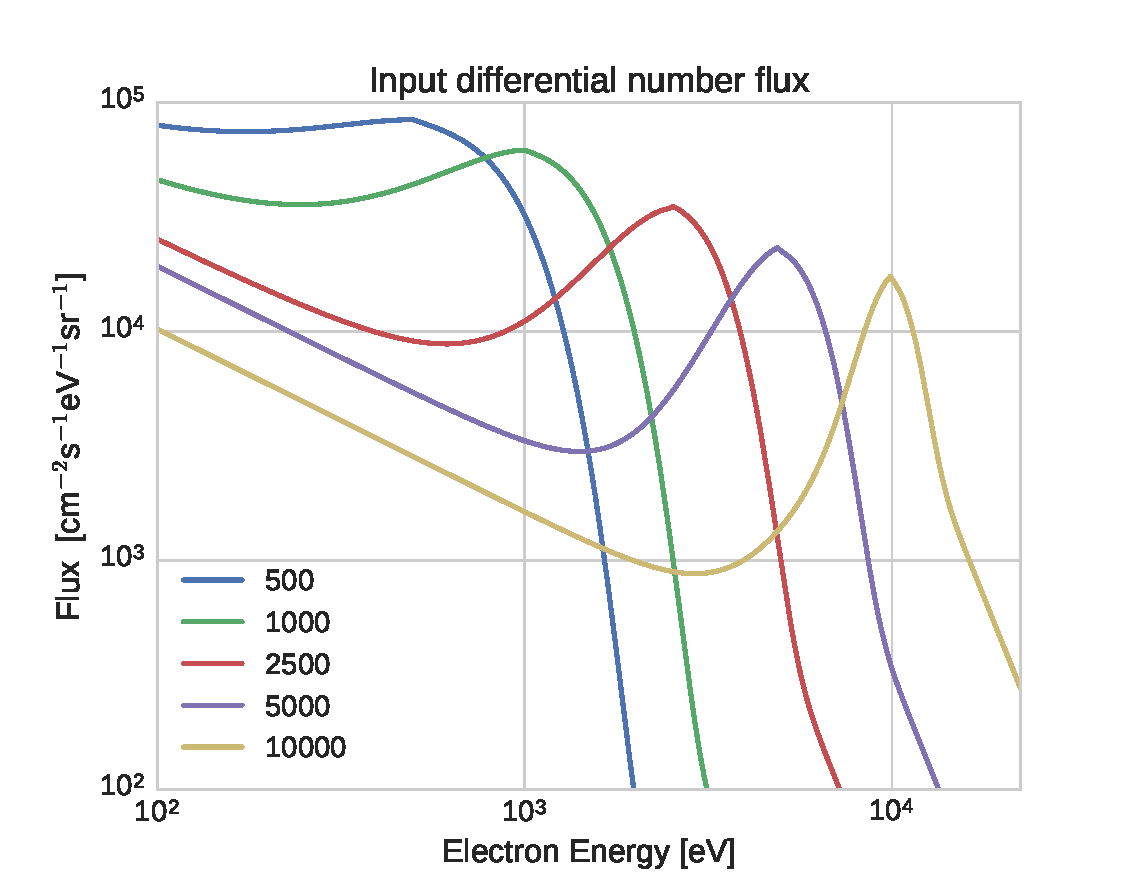
\includegraphics[width=\columnwidth,trim=0 0 50 20,clip]{gfx/hirsc6}
    \caption{Input differential number flux for beams with $E_0\in$ \{500, 1000, 2500, 5000, 10000\}~eV \citep{strickland1993}.}\label{fig:fwdstrick}
\end{figure}
%
The physical process generating $p_\lambda(z)$ in the second block of the left column of Figure~\ref{fig:overall} is modeled in TRANSCAR \citep{zett2007,blelly1996a,lilensten2002} and represented by the eigenprofiles $\mathbf{T}$ in the upper right block of Figure~\ref{fig:overall}, with line-integrated modeled spectra for each beam energy shown with and without BG3 filtering in Figure~\ref{fig:spectra}.
%
% python test_calcemissions.py ~/code/histfeas/test/data/ 1613.5 -t 0 -m spectra1d
%
\begin{figure}
    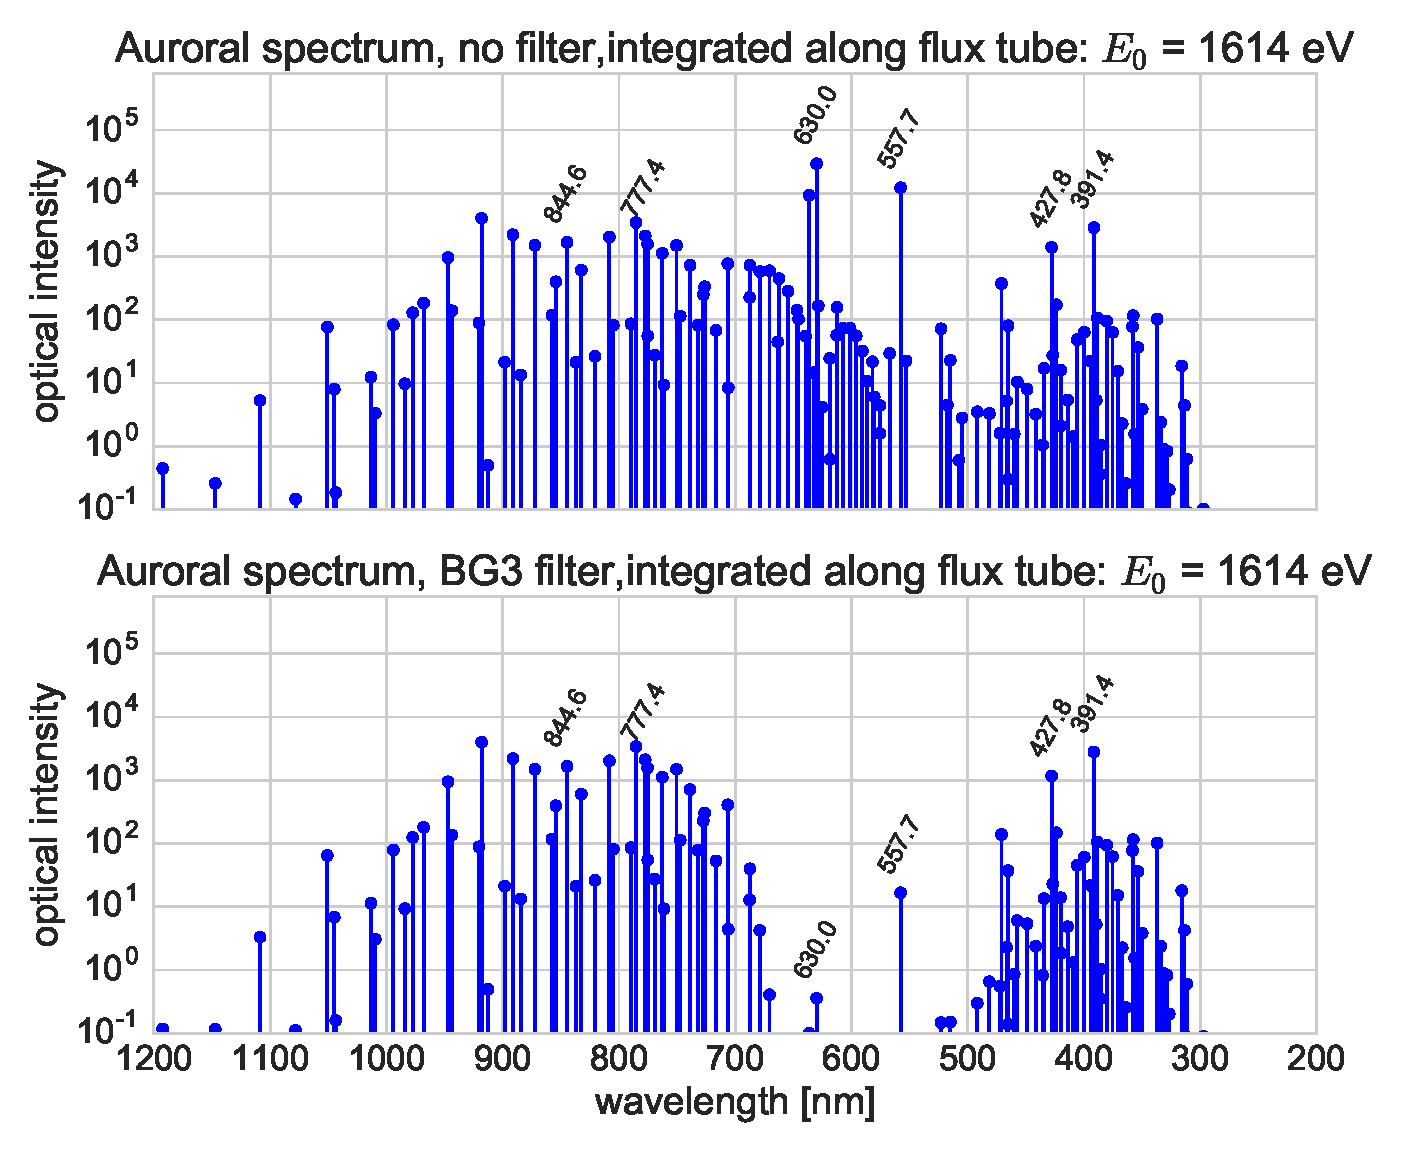
\includegraphics[width=\columnwidth,trim=0 10 0 0,clip]{gfx/hirsc7}
    \caption{Auroral Spectrum integrated along flux tube for $E_0=1.6$~keV, with and without BG3 filter.}\label{fig:spectra}
\end{figure} 
%
Some of the brightest features in the aurora are produced by metastable transitions with radiative lifetimes of order \unit[1..10]{s} \citep{vallancejones1974}. 
In Alfvénic aurora, the electron flux rapidly changes ($< \unit[10]{ms}$ scales) in $B_\perp$ and $E_0$, and the intense metastable emissions glow like an high-persistence oscilloscope phosphor, which in a white light sensor can cover up the much fainter prompt emissions that have several orders of magnitude shorter lifetimes.
Each camera was equipped with a BG3 optical filter with the transmission characteristics of Figure~\ref{fig:optTrans} to greatly attenuate these long lifetime features.
In particular, the deep notch in transmission for the long lifetime metastable emissions lines includes \unit[557.7]{nm} and \unit[630]{nm}.
%
% python gridaurora/test_opticalmod.py -m eps
\begin{figure}\centering
    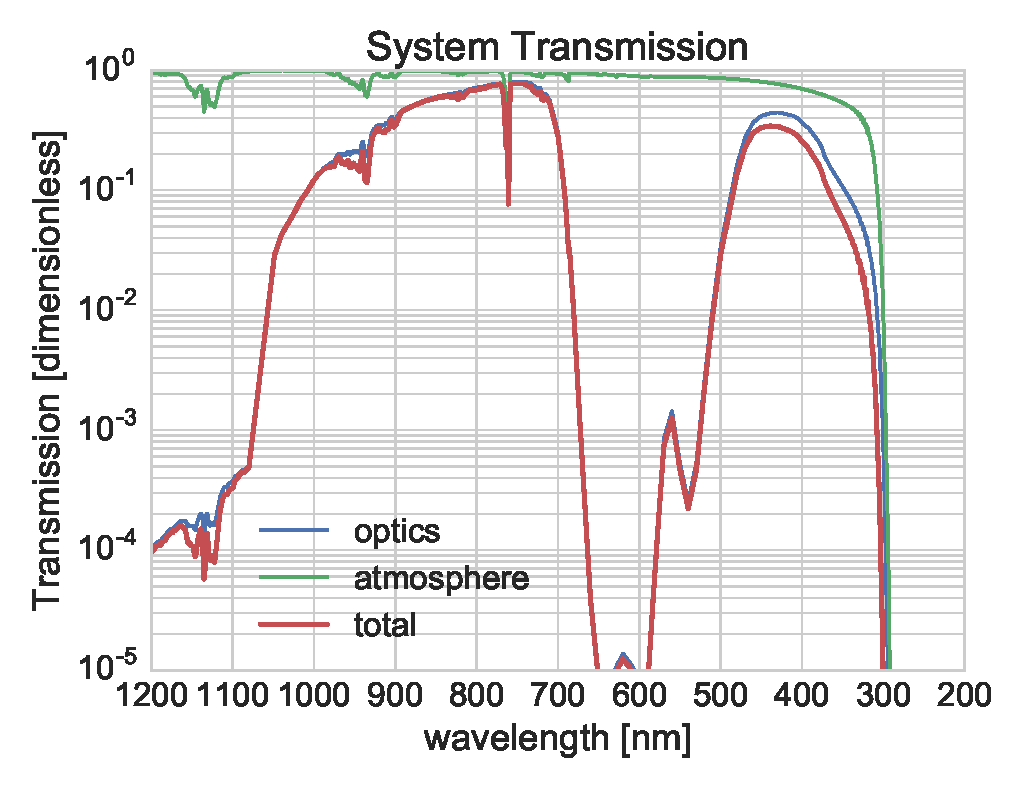
\includegraphics[width=\columnwidth,trim=5 5 5 5,clip]{gfx/hirsc8}
    \caption{Optical system transmission, including BG3 filter, EMCCD window and LOWTRAN modeled atmospheric absorption.}\label{fig:optTrans}
\end{figure}
%
The volume production rate of process $p_{ij}$ integrated over fixed pitch angle $\mu$ resulting from the TRANSCAR model is 
\begin{equation}\label{eq:prodEq2}
p_{ij}(z) =n_i(z) \int \sigma_{ij}(E)\Phi(z,E)\textrm{d}E 
\end{equation}
where $n_i$ is the MSIS90-initialized density of the i\textsuperscript{th} ground-state neutral species (e.g. N$_2$, O$_2$, O). $\sigma_{ij}$ is the electron impact cross section of the $j$\textsuperscript{th} excitation process for the $i$\textsuperscript{th} species \citep{semeter2012}. 
$\Phi(z,E)$ is the pitch angle integrated flux obtained from the 1-D model TRANSCAR \citep{blelly1996a} for 33 log-spaced energy bins $E$ ranging from \unit[58]{eV} to \unit[17.7]{keV} \citep{dahlgren2013}. 
For prompt emissions, we connect excitation rates to optical volume emission rates using~\eqref{eq:continuity} with \citep{zettdis,vallancejones1974} the Einstein coefficients and Franck-Condon factors,
\begin{equation}\label{eq:prompt4}
p_\lambda(z) \propto p_{ij}(z)
\end{equation}

For the lower left block of Figure~\ref{fig:overall}, the photon flux at the $k$\textsuperscript{th} camera pixel is described by a line integral mapped via the lens to angle $\theta_k$, treating the auroral region as optically thin at the wavelengths observable through the optical filtering and LOWTRAN \citep{lowtran7} modeled atmospheric absorption of Figure~\ref{fig:optTrans}.
Considering~\eqref{eq:prompt4} and total transmission $M(\lambda)$ shown in Figure~\ref{fig:optTrans}, the photon flux available at the imaging chip $\mathscr{I}(\theta)$ is
\begin{equation}\label{eq:grayb}
\mathscr{I}(\theta) =  \int_0^\infty \int_\lambda p(\lambda,\mathbf{\ell}) M(\lambda) \textrm{d} \lambda \textrm{d}\ell
\end{equation}
The camera exposure time $\tau$, amplifier gain $g$ and pixel area $a$ are modeled with the output in data numbers $\mathbf{I}$ as:
\begin{equation}\label{eq:dn}
\mathbf{I} = \tau a g \mathscr{I}
\end{equation}
where typical values include $a=(16~\mu\textrm{ m})^2, \tau = 2\times10^{-2}~\textrm{s}, g=1~I / \textrm{e}^- $.

Referring to the right column of Figure~\ref{fig:overall} we assemble projection matrix $\mathbf{L}$ by mapping viewing angle $\theta$ to our discrete EMCCD imaging arrays, and compute the intersection length of each ray \citep{semdis} with the relevant cell of $\mathbf{L}$ using the Cohen-Sutherland line clipping algorithm \citep{cohensutherland,cvutils}.
The dimensions of $\mathbf{L}$ are $N_{cam} N_{cut} \times N_{B_\perp} N_{B_\parallel}$,  where $N_{cam}$ is the number of cameras in the system, $N_{cut}$ is the number of 1-D pixels used from each camera and $N_{B_\perp},N_{B_\parallel}$ are the number of $B_\perp, B_\parallel$ pixels in the grid for the volume emission rate matrix $\mathbf{P}$ .
The IGRF 11 model is incorporated into $\mathbf{L}$ for the Poker Flat Research Range, where the inclination $77.5^\circ$ and declination $19.9^\circ$ of the local geomagnetic field determine the angular coördinates of magnetic zenith. 

The grid of Figure~\ref{fig:Lcam} extends from approximately 90-1000~km altitude, showing the locations used in estimating volume emission rate $\mathbf{P}$ due to the incident differential number flux $\Phi_{top}$.
\begin{figure}
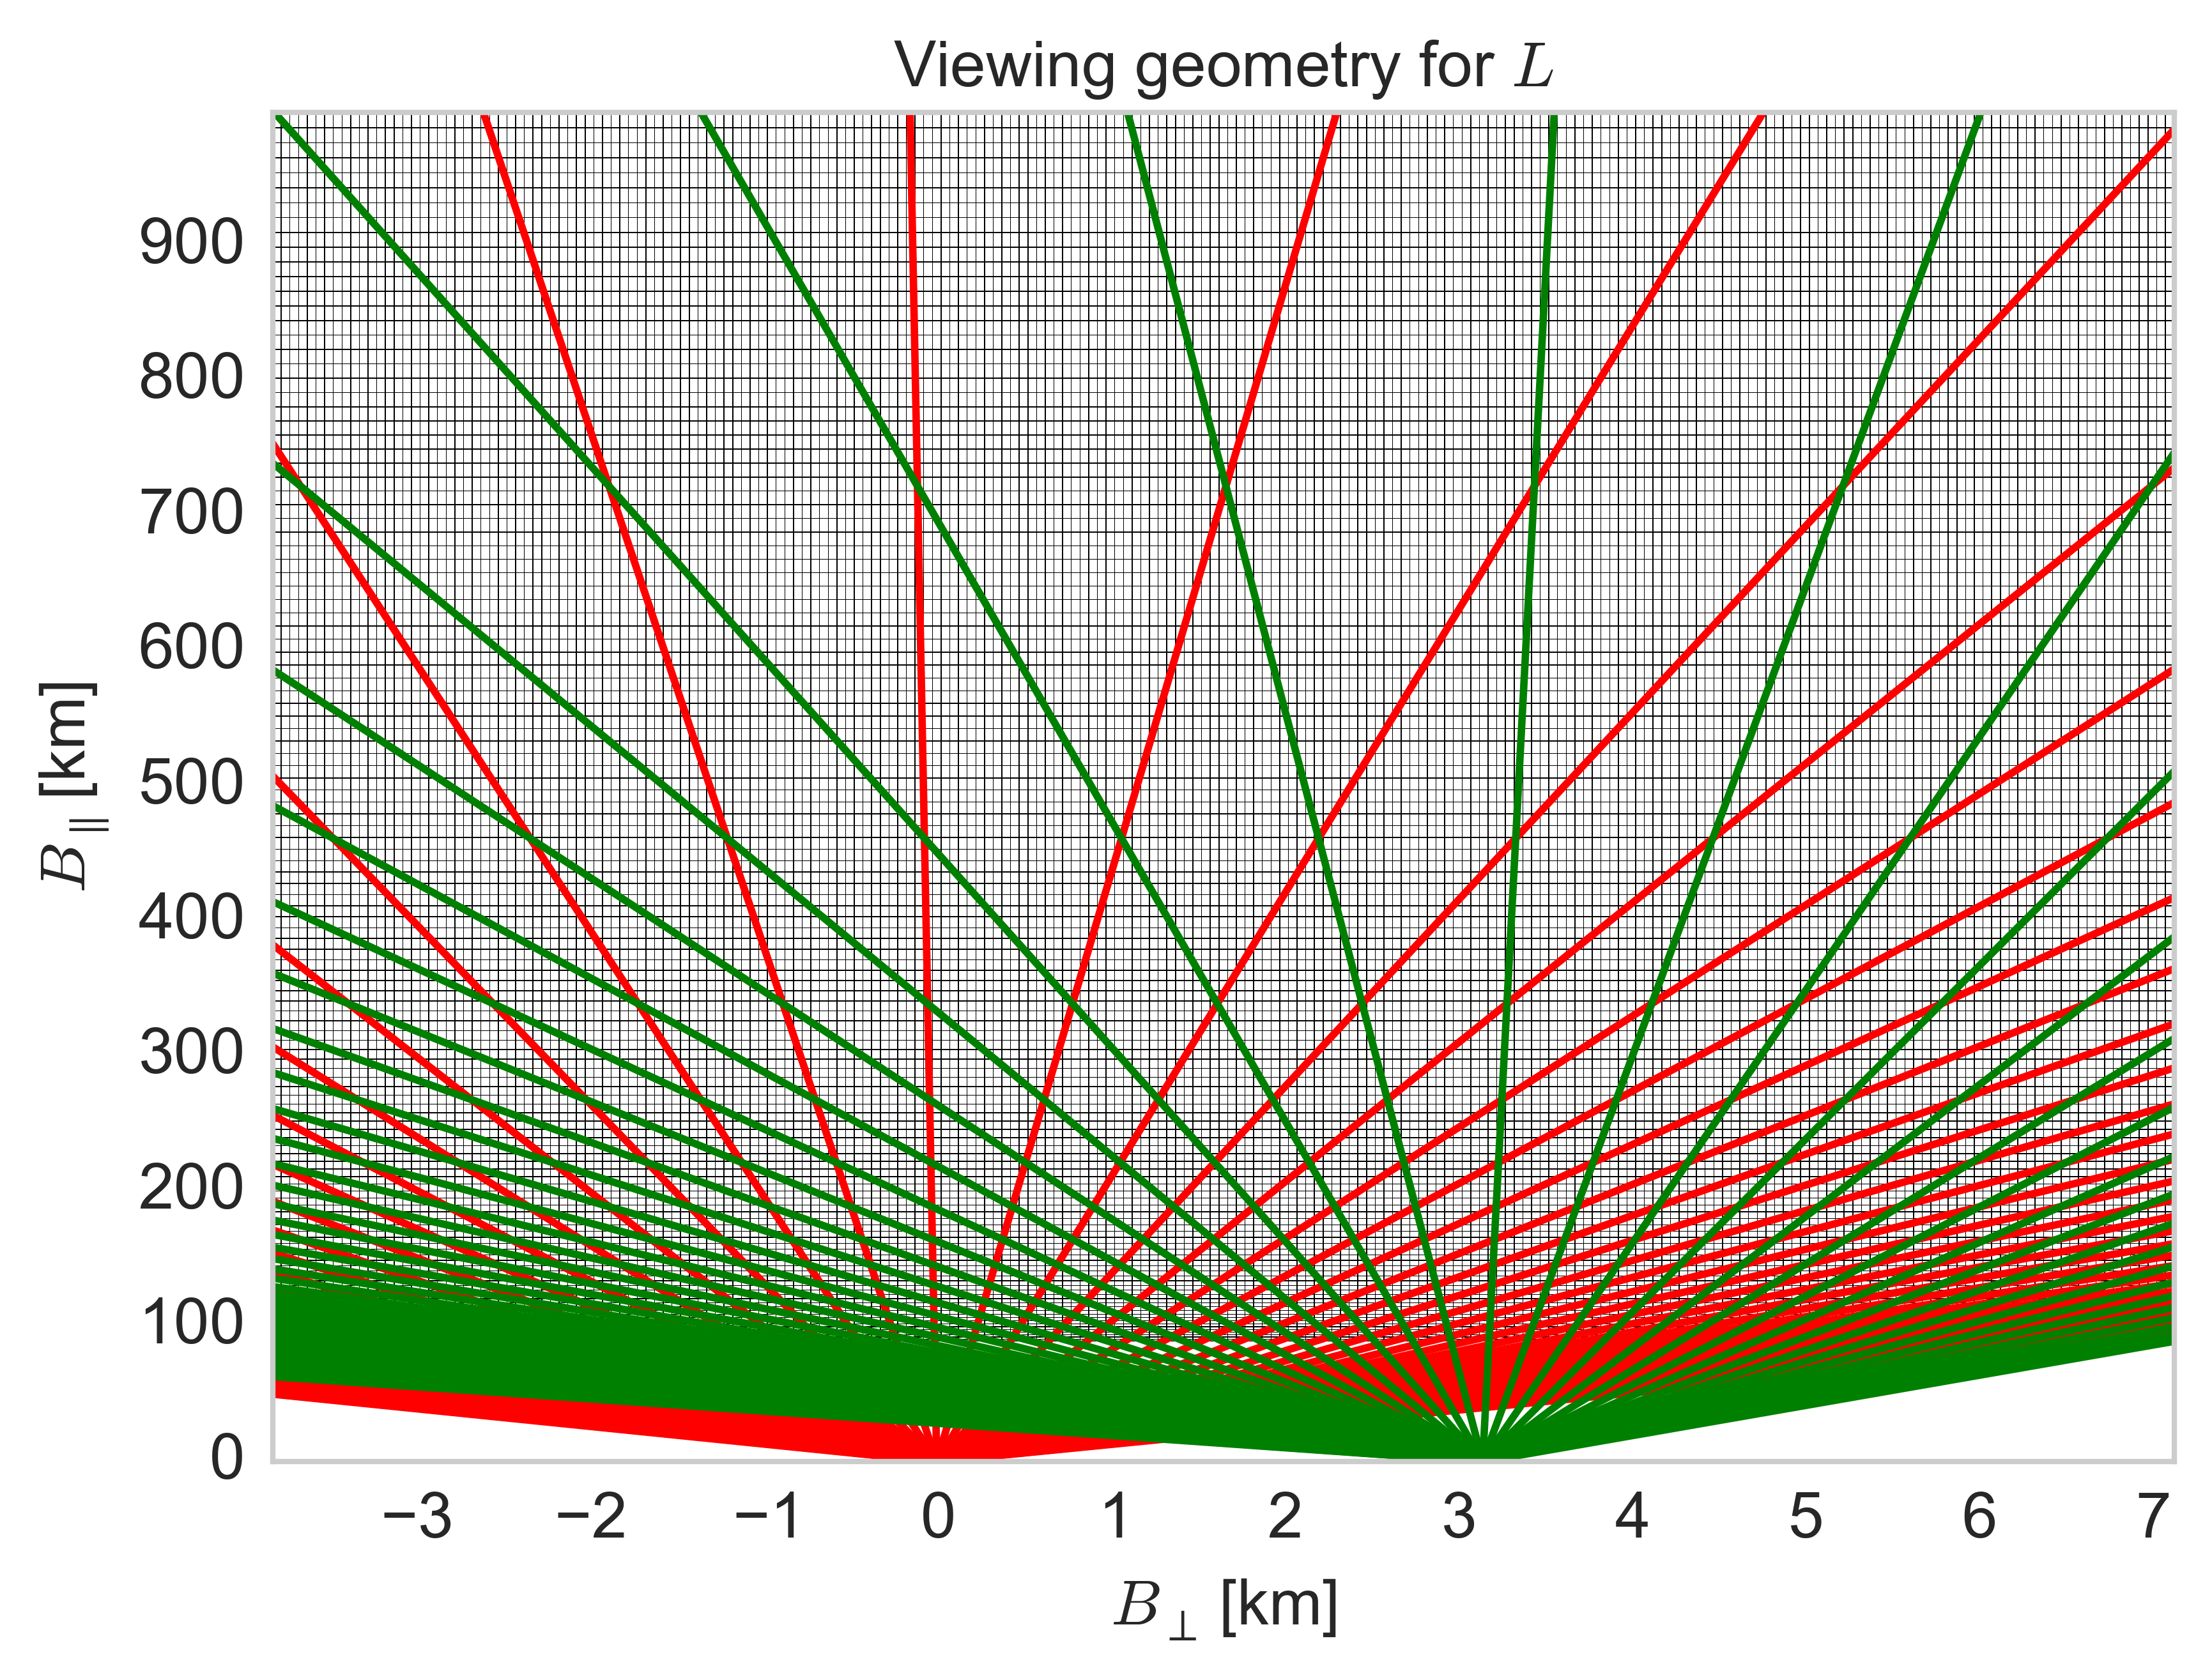
\includegraphics[width=\columnwidth,trim=5 6 5 5,clip]{gfx/Lcam}
\caption{Viewing geometry for the two-camera system at the Poker Flat Research Range, showing selected lines of sight over a decimated reconstruction grid.}\label{fig:Lcam}
\end{figure}
Overlaid on this grid are the decimated 1-D rays corresponding to intensity vector $\mathbf{I(\theta)}$.
For Figure~\ref{fig:Lcam} and the analysis of Section~\ref{sec:transverse} and~\ref{sec:flame}, $N_{cam}=2, N_{cut}=512, N_{B_\perp}=219, N_{B_\parallel}=123$.
This forward model yields ground-observed optical intensity vs. angle due to electron differential number flux $\Phi_{top}(B_\perp,E)$. 
The analysis in Section~\ref{sec:inv} uses observations from ground-based cameras to estimate the unobservable differential number flux $\hat{\Phi}_{top}$ via a minimization algorithm. 
